\subsection{A conditional flow for hydrogen coordinates}\label{app:hydrogen-readout}
A connected heavy-atom skeleton can still fail molecular validation if a hydrogen
lies too far from every heavy atom. In 512 cached training outputs per generator,
FM produces 346 connected heavy skeletons and GAGA 314, but hydrogen-only
fragmentation affects 60 FM outputs and 18 GAGA outputs. This motivates a
conditional coordinate model that holds the heavy-atom geometry fixed and
learns how the hydrogens should be arranged around it. Hydrogen decoration is
also supported by existing generators such as Quetzal
\citep{cheng2025quetzal}; here we test it as a selective readout of a generated
structure, with explicit geometric and physical controls.

\paragraph{Inputs, targets, and training.}
The model receives all current coordinates, atomic numbers, and a completion
time $s\in[0,1]$. Its output is a three-dimensional velocity for each hydrogen.
For a training structure, we perturb hydrogen coordinates with Gaussian noise
of standard deviation 0.4\,\AA, keeping heavy atoms fixed. Half of the examples
perturb every hydrogen; the other half perturb each hydrogen independently with
probability one half. We pair perturbed and reference hydrogen positions by
minimum squared-distance assignment, so the target does not depend on arbitrary
labels of identical hydrogens. If $Y_0$ denotes the perturbed hydrogen coordinates
and $Y_1$ their assigned reference positions, the training path and loss are
\begin{equation}
 Y_s=(1-s)Y_0+sY_1,\qquad
 \mathcal L_H=\EE\!\left[\frac{1}{3N_H}
 \left\|u_\psi(X_{\rm heavy},Y_s,s;z)-(Y_1-Y_0)\right\|_F^2\right].
\end{equation}
Here $X_{\rm heavy}$ contains the fixed heavy-atom coordinates, $z$ lists all
atomic numbers, $N_H$ is the hydrogen count, and $u_\psi$ is the predicted
hydrogen velocity. A common translation centers the full input; it does not
change relative coordinates. Training uses coordinates and atom identities,
without bond labels, energies, or forces.

We use a four-layer, width-64 EGNN with 153,790 total parameters, including
1,001 frozen schedule entries. Two independently initialized models each train
for 10,000 updates of batch size 32 on the same 20,000 OMol25 structures used
by the shared-backbone generators. The learning rate is $3\cdot10^{-4}$ and
the exponential moving average decay is 0.999. We use the final averaged
checkpoint. These fits add 640,000 training-example forward passes in total;
the same two hydrogen models serve both FM and GAGA.

\paragraph{Generation and controls.}
The parent generators use their frozen strength-four physical corrections.
A hydrogen activates the readout when its distance from every heavy atom
exceeds 1.25 times their summed covalent radii. With no such hydrogen, the
entire output is unchanged. Otherwise we integrate the conditional flow from
$s=0$ to $1$, allowing all hydrogens in that molecule to move. Four midpoint
steps require eight small-network evaluations per activated output. Each
predicted hydrogen velocity is capped at 2\,\AA\ per unit completion time.
Heavy atoms remain fixed during integration, and a final common translation
restores the input centroid. Thus their relative geometry is preserved.
No force or energy evaluator is called during this readout.

The fixed radial control moves each detached hydrogen toward its nearest heavy
atom until their separation equals the sum of covalent radii. It leaves all
other relative coordinates fixed. A second control applies the learned flow
only to the hydrogens that triggered the readout, instead of moving all
hydrogens together. Both controls start from exactly the same parent outputs.
These are coordinate readouts, distinct from both the unchanged parent and
force-field or quantum geometry optimization.

\paragraph{Selection and independent physical test.}
Sixteen development compositions compare the radial rule with the two learned
modes, each starting at time zero or one half. Moving all hydrogens from time
zero gives the highest FM joint yield, 96/256 versus the radial rule's 95/256,
but does not meet the requirement of improvement in both fits. Its lower
energy motivates a separate physical hypothesis: relative to the radial rule,
the learned readout lowers mean energy per atom while retaining pooled graph
and joint yield. This hypothesis and the frozen model are specified before
generation on 30 new compositions, 15 each with 17--28 and 29--40 atoms.
Each fit draws 16 samples per composition, giving 960 attempts per setting.
Composition bootstrap intervals retain both fitted models in every resample.

\begin{table}[h]
\centering\small
\caption{Hydrogen readouts on 30 fresh compositions. All rows use the same
strength-four physical heads. Joint yield additionally requires GFN2 force
RMS at most 5 eV/\AA. Energy is the all-output change relative to the
corresponding unchanged parent, in meV/atom.}
\begin{tabular}{llrrr}
\toprule
Parent & Hydrogen readout & Graph (\%) & Joint (\%) & Energy change\\
\midrule
FM & None &25.31&24.17&0\\
FM & Radial rule &27.29&25.94&$+1.89$\\
FM & Conditional flow &27.40&26.04&$-13.32$\\
GAGA & None &23.85&23.54&0\\
GAGA & Radial rule &24.06&23.75&$+1.05$\\
GAGA & Conditional flow &24.06&23.75&$-2.04$\\
\bottomrule
\end{tabular}\label{tab:hydrogen-readout}
\end{table}

For FM, the learned readout lowers energy by 15.21 meV/atom relative to the
radial rule (95\% interval for the reduction $[10.10,21.71]$), with reductions
in both fits. Graph and joint yield each differ by only $+0.10$ percentage
points ($[-0.21,0.42]$). Relative to the unchanged parent, graph validity
increases by 2.08 points ($[1.15,3.13]$) and joint yield by 1.88 points
($[1.04,2.71]$). Every previously graph-valid parent remains unchanged.
Allowing all hydrogens to move, rather than only the detached ones, further
reduces energy by 10.25 meV/atom ($[6.96,14.72]$), with identical graph and
joint counts. This ablation supports learning their arrangement together.
GAGA also benefits physically: its learned readout lowers energy by
3.10 meV/atom relative to the radial rule ($[1.04,6.34]$).

With the same learned readout for both generators, FM exceeds GAGA in graph
validity by 3.33 points ($[0.52,6.15]$). The joint difference is $+2.29$ points
($[-0.63,5.21]$), so this physical-quality ordering remains uncertain.
The all-output energy averages include invalid geometries. As a descriptive
check on valid outputs, 261 paired FM structures pass graph validation under
both readouts; 18 are newly repaired. On these 18 pairs the learned readout
has 83.81 meV/atom lower mean energy than the radial rule. This conditional
subset is not used for model selection or for the primary energy interval.

\begin{figure}[t]
\centering
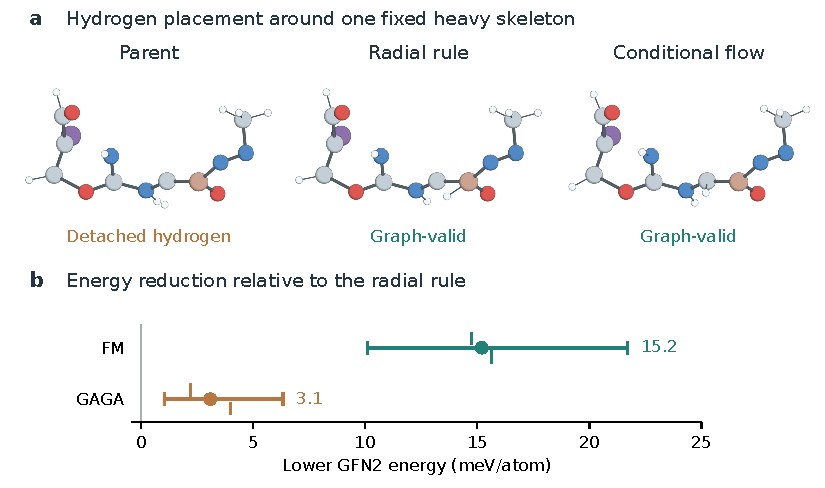
\includegraphics[width=\linewidth]{../research/figures/hydrogen_readout_v1/hydrogen_readout.pdf}
\caption{A conditional hydrogen flow learns more than attachment distance.
Top: the same saved FM output before readout, after the radial rule, and after
the learned flow. All atoms are shown with a shared camera and scale. Sticks
are distance contacts in every panel, not inferred chemical bond orders.
The example is selected by a fixed metadata hash among repaired, jointly
graph-valid examples with at most 28 atoms; energy is not a selection criterion.
Bottom: all-output energy reductions relative to the radial rule, with
95\% composition-bootstrap intervals and the two fit-specific means.
Carbon, hydrogen, nitrogen, oxygen, boron, and iodine are gray, white, blue, red,
tan, and purple.}\label{fig:hydrogen-readout}
\end{figure}

The confirmation generates 1,920 parent trajectories and 5,760 derived outputs.
It requires 2,460 new GFN2 calculations: one per parent and 540 unique changed
geometries. Identical coordinates reuse the original calculation. These costs
are separate from development, which uses 2,560 derived outputs and 155 new
GFN2 calculations, and from fitting the hydrogen models. All sampled outputs
remain in the reported denominators. The result establishes a local physical
benefit of the readout, not sampling from a global Boltzmann distribution.
